\begin{flushleft}
	{\color{blue!50!green}\fbox{\fontfamily{qag}\bfseries\selectfont PHẦN I. Câu trắc nghiệm nhiều phương án lựa chọn}}
	\textit{\small (Thí sinh trả lời từ câu 1 đến câu 18. Mỗi câu hỏi thí sinh chỉ chọn một phương án.)}
\end{flushleft}
\setcounter{ex}{0}
\setcounter{bt}{0}

% Câu 1
\begin{ex}
	\macau{ID: VL10-NH101-C01}Đối tượng nghiên cứu của Vật lí là
	\choice
	{sự thay đổi của các chất khi kết hợp với nhau}
	{qui luật tương tác của các dạng năng lượng}
	{nghiên cứu về nhiệt động lực học}
	{\True các dạng vận động của vật chất và năng lượng}
	\loigiai{
		Vật lí là môn khoa học tự nhiên có đối tượng nghiên cứu tập trung vào các dạng vận động cơ bản của vật chất và năng lượng, cũng như quy luật tương tác giữa chúng.
	}
\end{ex}

% Câu 2
\begin{ex}
	\macau{ID: VL10-NH101-C02}Một vật rơi tự do từ độ cao $80\text{ m}$ xuống đất. Lấy $g = 10\text{ m/s}^2$, tốc độ vật lúc vừa chạm đất là
	\choice
	{\True $40\text{ m/s}$}
	{$20\text{ m/s}$}
	{$10\text{ m/s}$}
	{$30\text{ m/s}$}
	\loigiai{
		Tốc độ của vật khi vừa chạm đất sau khi rơi tự do từ độ cao $h = 80\text{ m}$ là:
		\[
		v = \sqrt{2gh} = \sqrt{2 \cdot 10 \cdot 80} = \sqrt{1600} = 40\text{ m/s}.
		\]
	}
\end{ex}

% Câu 3
\begin{ex}
	\macau{ID: VL10-NH101-C03}Sự rơi tự do là
	\choice
	{\True chuyển động chỉ dưới tác dụng của trọng lực}
	{một dạng chuyển động thẳng đều}
	{chuyển động khi bỏ qua mọi lực}
	{chuyển động không chịu bất cứ lực tác dụng nào}
	\loigiai{
		Theo định nghĩa trong SGK Vật lí 10, sự rơi tự do là chuyển động của một vật chỉ chịu tác dụng duy nhất của trọng lực (khi bỏ qua sức cản không khí).
	}
\end{ex}

% Câu 4
\begin{ex}
	\macau{ID: VL10-NH101-C04}Trong chuyển động thẳng biến đổi đều thì
	\choice
	{vận tốc là đại lượng biến thiên theo thời gian theo quy luật hàm bậc hai}
	{\True gia tốc là đại lượng không đổi}
	{vận tốc là đại lượng không đổi}
	{gia tốc là đại lượng biến thiên theo thời gian}
	\loigiai{
		Chuyển động thẳng biến đổi đều là chuyển động thẳng có gia tốc không đổi theo thời gian ($a = \text{const}$). Vận tốc biến thiên theo hàm bậc nhất của thời gian: $v = v_0 + at$.
	}
\end{ex}

% Câu 5
\begin{ex}
	\macau{ID: VL10-NH101-C05}Gia tốc là một đại lượng
	\choice
	{vô hướng, đặc trưng cho sự biến đổi nhanh hay chậm của chuyển động}
	{vectơ, đặc trưng cho sự biến đổi nhanh hay chậm của chuyển động}
	{vô hướng, đặc trưng cho tính không đổi của vận tốc}
	{\True vectơ, đặc trưng cho sự biến đổi nhanh hay chậm của vận tốc}
	\loigiai{
		Gia tốc là một đại lượng vectơ đặc trưng cho sự biến đổi nhanh hay chậm của vận tốc theo thời gian, được xác định bằng:
		\[
		\vec{a} = \frac{\Delta \vec{v}}{\Delta t}.
		\]
	}
\end{ex}

% Câu 6
\begin{ex}
	\macau{ID: VL10-NH101-C06}Canô chuyển động thẳng xuôi dòng từ P đến Q mất 2 giờ và ngược dòng từ Q về P mất 3 giờ. Khi nước yên lặng canô chuyển động có tốc độ $50\text{ km/h}$. Tốc độ của nước so với bờ là
	\choice
	{$12{,}5\text{ km/h}$}
	{$9\text{ km/h}$}
	{\True $10\text{ km/h}$}
	{$20\text{ km/h}$}
	\loigiai{
		Gọi $s$ là khoảng cách giữa hai bến P và Q ($s > 0$). Tốc độ của canô đối với nước là $v_c = 50\text{ km/h}$, tốc độ dòng nước so với bờ là $v_n$ ($0 < v_n < 50$).\\
		Khi xuôi dòng: $v_{\text{xuôi}} = v_c + v_n = 50 + v_n \implies s = 2(50 + v_n)$.\\
		Khi ngược dòng: $v_{\text{ngược}} = v_c - v_n = 50 - v_n \implies s = 3(50 - v_n)$.\\
		Vì quãng đường không đổi:
		\[
		2(50 + v_n) = 3(50 - v_n) \iff 100 + 2v_n = 150 - 3v_n \iff 5v_n = 50 \iff v_n = 10\text{ km/h}.
		\]
	}
\end{ex}

% Câu 7
\begin{ex}
	\macau{ID: VL10-NH101-C07}Kí hiệu \raisebox{-0.35\height}{
\includegraphics[height=1.05cm]{c7_rac.png}} mang ý nghĩa gì?
	\choice
	{\True Không được phép bỏ vào thùng rác}
	{Tránh ánh nắng chiếu trực tiếp}
	{Dụng cụ dễ vỡ}
	{Dụng cụ cần đặt đứng}
	\loigiai{
		Biểu tượng thùng rác có bánh xe bị gạch chéo (WEEE Symbol) là biển cảnh báo đối với các thiết bị điện và điện tử, chỉ dẫn rằng không được vứt bỏ thiết bị cùng với rác thải sinh hoạt thông thường mà phải được thu gom, phân loại và xử lý riêng biệt.
	}
\end{ex}

% Câu 8
\begin{ex}
	\macau{ID: VL10-NH101-C08}Đồ thị độ dịch chuyển -- thời gian trong chuyển động thẳng của một chất điểm có dạng như hình vẽ. Trong thời gian nào xe chuyển động thẳng đều?
	\begin{center}
		\vspace{-7pt}
		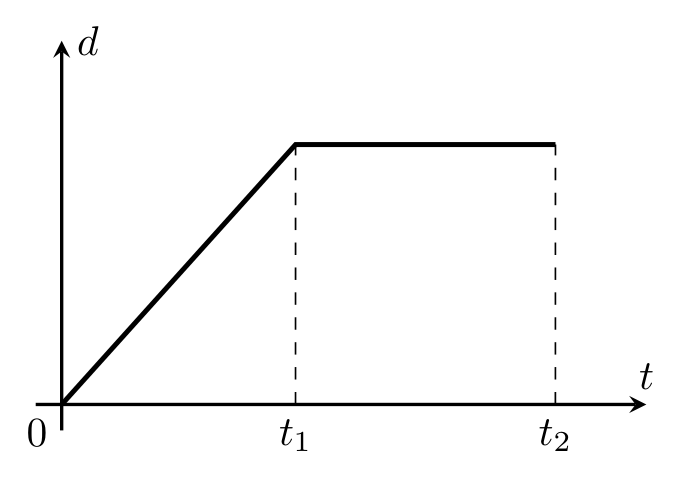
\includegraphics[width=3.8cm]{c8_dothidt.png}
		\vspace{-7pt}
	\end{center}
	\choice
	{Không có lúc nào xe chuyển động thẳng đều}
	{\True Trong khoảng thời gian từ $0$ đến $t_1$}
	{Trong khoảng thời gian từ $t_1$ đến $t_2$}
	{Trong khoảng thời gian từ $0$ đến $t_2$}
	\loigiai{
		Trên đồ thị độ dịch chuyển -- thời gian ($d - t$):\\
		- Trong khoảng thời gian từ $0$ đến $t_1$, đồ thị là đường thẳng xiên dốc lên xuất phát từ gốc tọa độ, hệ số góc không đổi $v = \dfrac{\Delta d}{\Delta t} > 0$, biểu diễn chuyển động thẳng đều.\\
		- Trong khoảng thời gian từ $t_1$ đến $t_2$, đồ thị là đường nằm ngang ($d = \text{const}$), biểu diễn chất điểm đứng yên.
	}
\end{ex}

% Câu 9
\begin{ex}
	\macau{ID: VL10-NH101-C09}Phát biểu nào sau đây \textbf{không đúng}?
	\choice
	{Độ dịch chuyển là vectơ nối vị trí đầu và vị trí cuối của chất điểm chuyển động}
	{Chất điểm đi trên một đường thẳng rồi quay về vị trí ban đầu thì có độ dịch chuyển bằng không}
	{\True Độ dịch chuyển bằng quãng đường đi được của chất điểm}
	{Độ dịch chuyển là đại lượng vectơ còn quãng đường đi được là đại lượng vô hướng}
	\loigiai{
		Độ lớn của độ dịch chuyển chỉ bằng quãng đường đi được ($d = s$) khi chất điểm chuyển động thẳng và không đổi chiều. Trong chuyển động có đổi chiều hoặc chuyển động cong thì $d < s$. Do đó phát biểu "Độ dịch chuyển bằng quãng đường đi được của chất điểm" là không đúng.
	}
\end{ex}

% Câu 10
\begin{ex}
	\macau{ID: VL10-NH101-C10}Dùng thước đo có sai số dụng cụ là $1\text{ mm}$ để đo 5 lần khoảng cách giữa hai điểm M và N đều cho một giá trị như nhau là $56\text{ mm}$. Kết quả của phép đo được viết là
	\choice
	{$d = 56 \pm 0\text{ mm}$}
	{$d = 56 \pm 2\text{ mm}$}
	{\True $d = 56 \pm 1\text{ mm}$}
	{$d = 56 \pm 0{,}5\text{ mm}$}
	\loigiai{
		Giá trị trung bình của phép đo là $\overline{d} = 56\text{ mm}$. Vì cả 5 lần đo đều ra cùng giá trị $56\text{ mm}$ nên sai số ngẫu nhiên $\overline{\Delta d} = 0$. Sai số tuyệt đối của phép đo bằng sai số dụng cụ: $\Delta d = \Delta d_{dc} = 1\text{ mm}$.\\
		Kết quả phép đo được viết là: $d = \overline{d} \pm \Delta d = 56 \pm 1\text{ mm}$.
	}
\end{ex}

% Câu 11
\begin{ex}
	\macau{ID: VL10-NH101-C11}Trong các chuyển động sau, chuyển động nào được coi là sự rơi tự do?
	\choice
	{Chiếc lá đang rơi}
	{Hạt bụi chuyển động trong không khí}
	{Vận động viên đang nhảy dù}
	{\True Quả tạ rơi trong không khí từ độ cao $50\text{ m}$}
	\loigiai{
		Khi một vật rơi trong không khí mà lực cản của không khí rất nhỏ không đáng kể so với trọng lượng của vật thì sự rơi đó được coi gần đúng là sự rơi tự do. Quả tạ đặc bằng kim loại có trọng lượng rất lớn so với lực cản không khí nên chuyển động rơi của nó được coi là rơi tự do.
	}
\end{ex}

% Câu 12
\begin{ex}
	\macau{ID: VL10-NH101-C12}Một ô tô đang chuyển động cùng chiều dương với tốc độ $10\text{ m/s}$ trên đoạn đường thẳng thì người lái xe hãm phanh và ô tô chuyển động chậm dần đều. Cho tới khi dừng hẳn thì ô tô đã chạy thêm được $100\text{ m}$. Gia tốc của xe có giá trị bằng
	\choice
	{$-0{,}2\text{ m/s}^2$}
	{\True $-0{,}5\text{ m/s}^2$}
	{$0{,}2\text{ m/s}^2$}
	{$0{,}5\text{ m/s}^2$}
	\loigiai{
		Áp dụng công thức độc lập với thời gian: $v^2 - v_0^2 = 2as$.\\
		Với $v_0 = 10\text{ m/s}$, $v = 0$ (khi dừng hẳn), quãng đường $s = 100\text{ m}$:\\
		\[
		0^2 - 10^2 = 2 \cdot a \cdot 100 \iff -100 = 200a \implies a = -0{,}5\text{ m/s}^2.
		\]
	}
\end{ex}

% Câu 13
\begin{ex}
	\macau{ID: VL10-NH101-C13}Một vật được thả rơi tự do, tốc độ của vật khi chạm đất là $70\text{ m/s}$. Cho $g = 10\text{ m/s}^2$. Thời gian vật rơi là
	\choice
	{$3{,}5\text{ s}$}
	{\True $7\text{ s}$}
	{$8\text{ s}$}
	{$4\text{ s}$}
	\loigiai{
		Thời gian vật rơi tự do được tính từ công thức vận tốc:
		\[
		v = gt \implies t = \frac{v}{g} = \frac{70}{10} = 7\text{ s}.
		\]
	}
\end{ex}

% Câu 14
\begin{ex}
	\macau{ID: VL10-NH101-C14}Chọn câu đúng. Để đo tốc độ trung bình của vật trong phòng thí nghiệm, ta cần dùng
	\choice
	{\True thước đo chiều dài và đồng hồ đo thời gian}
	{thước đo và lực kế}
	{máy bắn tốc độ}
	{lực kế và đồng hồ đo thời gian}
	\loigiai{
		Tốc độ trung bình được xác định theo công thức $v_{tb} = \dfrac{s}{t}$. Do đó, để đo tốc độ trung bình trong phòng thí nghiệm ta cần dùng thước đo chiều dài (đo quãng đường $s$) và đồng hồ bấm giây/đồng hồ hiện số (đo thời gian $t$).
	}
\end{ex}

% Câu 15
\begin{ex}
	\macau{ID: VL10-NH101-C15}Cặp đồ thị nào ở hình dưới đây là của chuyển động thẳng đều?
	\begin{center}
		\vspace{-7pt}
		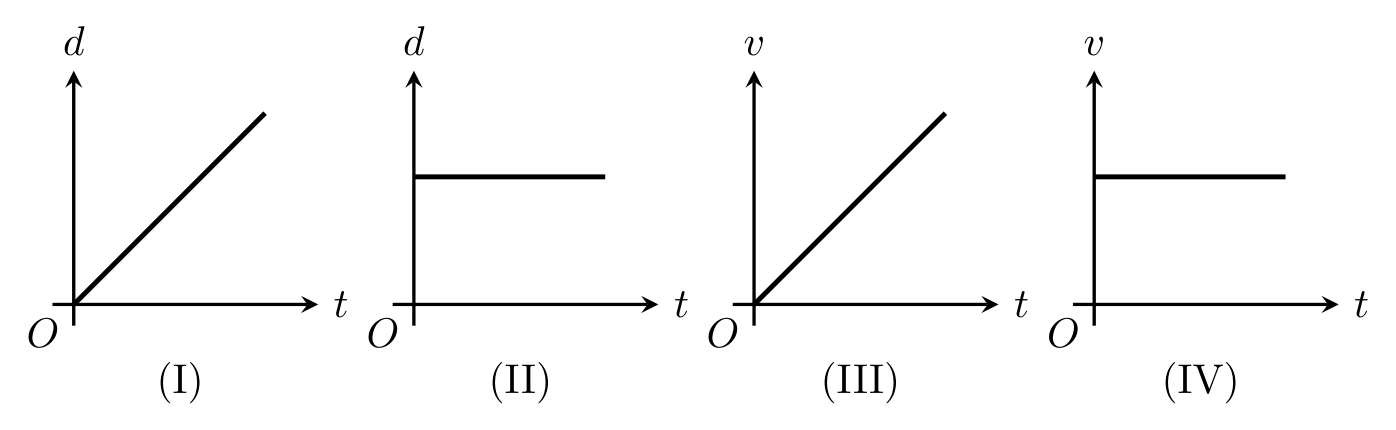
\includegraphics[width=11.5cm]{c15_dothi4.png}
		\vspace{-7pt}
	\end{center}
	\choice
	{I và III}
	{\True I và IV}
	{II và IV}
	{II và III}
	\loigiai{
		Trong chuyển động thẳng đều:\\
		- Vận tốc không đổi theo thời gian: $v(t) = \text{const}$, đồ thị $v - t$ là đường thẳng nằm ngang song song trục thời gian (hình IV).\\
		- Độ dịch chuyển tỉ lệ thuận với thời gian: $d(t) = v \cdot t$, đồ thị $d - t$ là đường thẳng đi qua gốc tọa độ (hình I).\\
		Vậy cặp đồ thị đúng là I và IV.
	}
\end{ex}

% Câu 16
\begin{ex}
	\macau{ID: VL10-NH101-C16}Vật chuyển động thẳng nhanh dần thì vectơ gia tốc và vectơ vận tốc
	\choice
	{ngược hướng}
	{\True cùng hướng}
	{không thay đổi}
	{vuông góc}
	\loigiai{
		Trong chuyển động thẳng nhanh dần, tốc độ của vật tăng theo thời gian nên tích $a \cdot v > 0$. Điều này có nghĩa là vectơ gia tốc $\vec{a}$ và vectơ vận tốc $\vec{v}$ luôn cùng hướng với nhau.
	}
\end{ex}

% Câu 17
\begin{ex}
	\macau{ID: VL10-NH101-C17}Câu trả lời nào sau đây \textbf{Sai}. Chuyển động thẳng nhanh dần đều là chuyển động có
	\choice
	{\True quãng đường đi được của vật luôn tỉ lệ thuận với thời gian vật đi}
	{quỹ đạo là đường thẳng}
	{vectơ gia tốc của vật có độ lớn là một hằng số}
	{vận tốc có độ lớn tăng theo hàm bậc nhất đối với thời gian}
	\loigiai{
		Phương trình quãng đường trong chuyển động thẳng nhanh dần đều có dạng $s = v_0 t + \dfrac{1}{2}at^2$, là hàm bậc hai theo thời gian, nên quãng đường không tỉ lệ thuận với thời gian. Do đó phát biểu A là sai.
	}
\end{ex}

% Câu 18
\begin{ex}
	\macau{ID: VL10-NH101-C18}Vào lúc $10\text{ h}$, người lái xe nhìn vào tốc kế và thấy tốc kế chỉ $40\text{ km/h}$. Số liệu này cho biết
	\choice
	{tốc độ trung bình của xe}
	{vận tốc trung bình của xe}
	{\True tốc độ tức thời của xe}
	{vận tốc tức thời của xe}
	\loigiai{
		Tốc kế (speedometer) gắn trên xe hiển thị độ lớn vận tốc của xe tại thời điểm quan sát, tức là tốc độ tức thời của xe.
	}
\end{ex}

\vspace{0.2cm}
\begin{flushleft}
	{\color{blue!50!green}\fbox{\fontfamily{qag}\bfseries\selectfont PHẦN II. Câu trắc nghiệm đúng sai}}
	\textit{\small (Thí sinh trả lời từ câu 1 đến câu 4. Trong mỗi ý a), b), c), d) ở mỗi câu, thí sinh chọn đúng hoặc sai.)}
\end{flushleft}
\setcounter{ex}{0}
\setcounter{bt}{0}

% Phần II Câu 1
\begin{ex}
	\macau{ID: VL10-NH101-C19}Hai bạn Đức và Triết bơi trong bể bơi có chiều dài $25\text{ m}$. Hai bạn xuất phát từ đầu bể bơi đến cuối bể bơi thì Đức dừng lại nghỉ, còn Triết quay lại và tiếp tục bơi tiếp về đầu bể bơi mới nghỉ. Thời gian bơi của Đức là $25\text{ s}$; Triết bơi đi mất $23\text{ s}$ và bơi về mất $27\text{ s}$. Biết rằng Đức và Triết bơi trên một đường thẳng song song với thành bể.
	\choiceTF
	{\True Tốc độ trung bình trong thời gian $25\text{ s}$ của Đức là $1\text{ m/s}$}
	{Vận tốc trung bình trong thời gian $50\text{ s}$ của Triết là $1\text{ m/s}$}
	{Độ dịch chuyển tổng hợp của Triết có độ lớn bằng $50\text{ m}$}
	{\True Quãng đường Đức bơi được là $25\text{ m}$}
	\loigiai{
		Chiều dài bể bơi là $L = 25\text{ m}$.
		\begin{itemize}
			\item Với Đức: Bơi từ đầu bể đến cuối bể rồi nghỉ. Quãng đường Đức bơi được là $s_{\text{Đ}} = 25\text{ m}$. Do đó ý d) \textbf{Đúng}.\\
			Thời gian bơi $t_{\text{Đ}} = 25\text{ s}$, nên tốc độ trung bình của Đức là:
			\[
			v_{tb(\text{Đ})} = \frac{s_{\text{Đ}}}{t_{\text{Đ}}} = \frac{25}{25} = 1\text{ m/s}.
			\]
			Do đó ý a) \textbf{Đúng}.
			\item Với Triết: Bơi từ đầu bể đến cuối bể ($25\text{ m}$) rồi quay lại đầu bể ($25\text{ m}$). Tổng quãng đường là $s_T = 25 + 25 = 50\text{ m}$. Tổng thời gian bơi là $t_T = 23 + 27 = 50\text{ s}$.\\
			Vì điểm xuất phát và điểm kết thúc của Triết trùng nhau (đều ở đầu bể bơi) nên độ dịch chuyển tổng hợp của Triết bằng $0\text{ m}$ (chứ không phải $50\text{ m}$). Do đó ý c) \textbf{Sai}.\\
			Vận tốc trung bình của Triết:
			\[
			v_{tb} = \frac{d_T}{t_T} = \frac{0}{50} = 0\text{ m/s} \ne 1\text{ m/s}.
			\]
			(Tốc độ trung bình mới bằng $1\text{ m/s}$). Do đó ý b) \textbf{Sai}.
		\end{itemize}
	}
\end{ex}

% Phần II Câu 2
\begin{ex}
	\macau{ID: VL10-NH101-C20}Một máy bay Boeing 747 bắt đầu xuất phát trên một đường băng thẳng dài với gia tốc $a = 2\text{ m/s}^2$. Tốc độ cần thiết để máy bay rời đường băng là $360\text{ km/h}$. Sau khi xuất phát được $30\text{ s}$ thì nhận được lệnh huỷ bay từ trạm điều khiển không lưu do thời tiết xấu nên phi công cho máy bay hãm phanh chuyển động chậm dần đều và dừng lại sau $20\text{ s}$ kể từ khi có lệnh huỷ bay.
	\choiceTF
	{\True Chuyển động của máy bay trong $30\text{ s}$ đầu tiên là chuyển động thẳng nhanh dần đều}
	{\True Tốc độ của máy bay tại thời điểm nhận được lệnh huỷ bay là $60\text{ m/s}$}
	{\True Độ lớn gia tốc của máy bay trong giai đoạn hãm phanh là $3\text{ m/s}^2$}
	{Tốc độ trung bình của máy bay trong khoảng thời gian từ lúc xuất phát cho đến khi dừng lại là $40\text{ m/s}$}
	\loigiai{
		\begin{itemize}
			\item Giai đoạn 1 ($30\text{ s}$ đầu): Vận tốc đầu $v_0 = 0$, gia tốc $a_1 = 2\text{ m/s}^2 > 0$. Vận tốc tăng dần đều theo thời gian nên đây là chuyển động thẳng nhanh dần đều. Do đó ý a) \textbf{Đúng}.\\
			Vận tốc tại thời điểm nhận lệnh huỷ bay ($t_1 = 30\text{ s}$):
			\[
			v_1 = v_0 + a_1 t_1 = 0 + 2 \cdot 30 = 60\text{ m/s}.
			\]
			Do đó ý b) \textbf{Đúng}.\\
			Quãng đường chạy trong $30\text{ s}$ đầu:
			\[
			s_1 = \frac{1}{2} a_1 t_1^2 = \frac{1}{2} \cdot 2 \cdot 30^2 = 900\text{ m}.
			\]
			\item Giai đoạn 2 (hãm phanh): Từ $v_1 = 60\text{ m/s}$ đến khi dừng hẳn $v_2 = 0$ trong thời gian $t_2 = 20\text{ s}$.\\
			Gia tốc của máy bay trong giai đoạn này:
			\[
			a_2 = \frac{v_2 - v_1}{t_2} = \frac{0 - 60}{20} = -3\text{ m/s}^2.
			\]
			Độ lớn gia tốc hãm phanh là $|a_2| = 3\text{ m/s}^2$. Do đó ý c) \textbf{Đúng}.\\
			Quãng đường hãm phanh:
			\[
			s_2 = \frac{v_1 + v_2}{2} \cdot t_2 = \frac{60 + 0}{2} \cdot 20 = 600\text{ m}.
			\]
			\item Toàn bộ quá trình:\\
			Tổng quãng đường: $s = s_1 + s_2 = 900 + 600 = 1500\text{ m}$.\\
			Tổng thời gian: $t = t_1 + t_2 = 30 + 20 = 50\text{ s}$.\\
			Tốc độ trung bình:
			\[
			v_{tb} = \frac{s}{t} = \frac{1500}{50} = 30\text{ m/s} \ne 40\text{ m/s}.
			\]
			Do đó ý d) \textbf{Sai}.
		\end{itemize}
	}
\end{ex}

% Phần II Câu 3
\begin{ex}
	\macau{ID: VL10-NH101-C21}Từ các đồ thị trong hình sau. Nhận định sau đúng hay sai?
	\begin{center}
		\vspace{-7pt}
		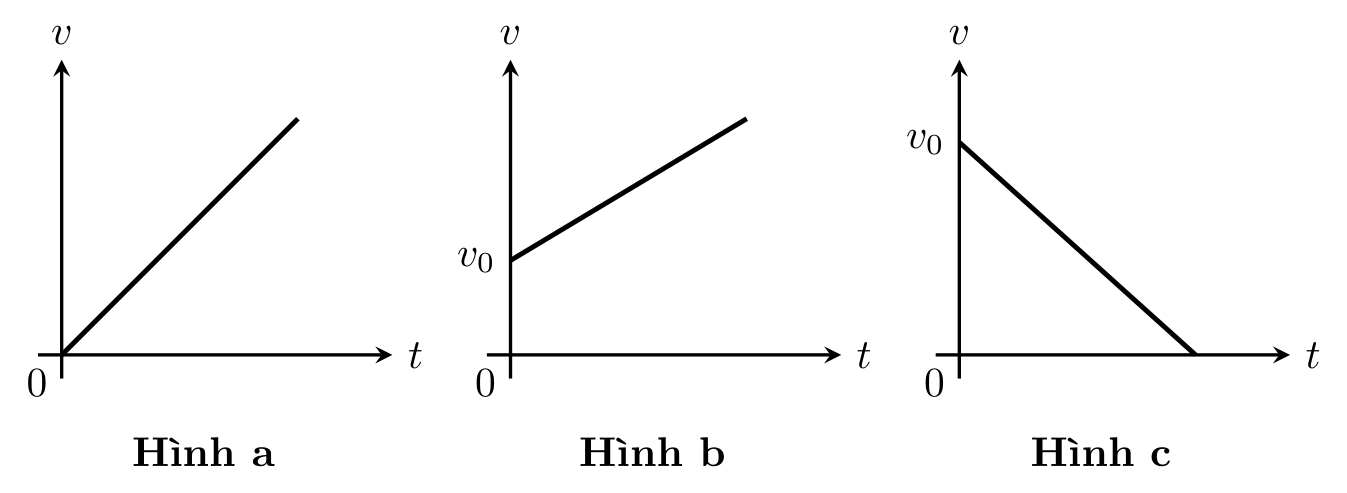
\includegraphics[width=10.5cm]{p2_c3_dothi3.png}
		\vspace{-7pt}
	\end{center}
	\choiceTF
	{\True Chuyển động thẳng nhanh dần đều là đồ thị hình a và b}
	{Đồ thị hình b có công thức vận tốc là $v = v_0 + at\ (a < 0)$}
	{\True Chuyển động thẳng chậm dần đều là đồ thị hình c}
	{Đồ thị hình c có công thức vận tốc là $v = v_0 + at\ (a > 0)$}
	\loigiai{
		\begin{itemize}
			\item Hình a và hình b: Đồ thị $v - t$ là đường thẳng dốc lên từ trái sang phải, vận tốc có độ lớn tăng đều theo thời gian, nên đây là chuyển động thẳng nhanh dần đều. Do đó ý a) \textbf{Đúng}.
			\item Ở hình b, đồ thị dốc lên nên hệ số góc $a = \dfrac{\Delta v}{\Delta t} > 0$. Công thức vận tốc phải có $a > 0$. Do đó ý b) \textbf{Sai}.
			\item Hình c: Đồ thị $v - t$ là đường thẳng dốc xuống từ $v_0$ về 0, độ lớn vận tốc giảm đều theo thời gian về 0, nên đây là chuyển động thẳng chậm dần đều. Do đó ý c) \textbf{Đúng}.
			\item Ở hình c, đồ thị dốc xuống nên hệ số góc $a = \dfrac{\Delta v}{\Delta t} < 0$. Công thức vận tốc phải có $a < 0$. Do đó ý d) \textbf{Sai}.
		\end{itemize}
	}
\end{ex}

% Phần II Câu 4
\begin{ex}
	\macau{ID: VL10-NH101-C22}Bỏ qua sức cản không khí, một vật rơi tự do tại một địa điểm có độ cao $180\text{ m}$, lấy $g = 10\text{ m/s}^2$.
	\choiceTF
	{Quãng đường vật rơi được sau $3\text{ s}$ là $30\text{ m}$}
	{\True Phương rơi của vật là phương thẳng đứng}
	{\True Thời gian vật rơi hết $100\text{ m}$ cuối cùng là $2\text{ s}$}
	{Thời gian vật rơi hết quãng đường là $9\text{ s}$}
	\loigiai{
		\begin{itemize}
			\item Tổng thời gian rơi tự do từ độ cao $h = 180\text{ m}$:
			\[
			t = \sqrt{\frac{2h}{g}} = \sqrt{\frac{2 \cdot 180}{10}} = \sqrt{36} = 6\text{ s}.
			\]
			Do đó thời gian vật rơi hết quãng đường là $6\text{ s}$ chứ không phải $9\text{ s}$. Ý d) \textbf{Sai}.
			\item Quãng đường vật rơi được sau $3\text{ s}$:
			\[
			s_3 = \frac{1}{2} g t_3^2 = \frac{1}{2} \cdot 10 \cdot 3^2 = 45\text{ m} \ne 30\text{ m}.
			\]
			Do đó ý a) \textbf{Sai}.
			\item Chuyển động rơi tự do luôn có phương thẳng đứng, chiều hướng từ trên xuống dưới. Do đó ý b) \textbf{Đúng}.
			\item Để rơi hết $100\text{ m}$ cuối cùng, trước đó vật rơi quãng đường là:
			\[
			s_1 = 180 - 100 = 80\text{ m}.
			\]
			Thời gian để rơi $80\text{ m}$ đầu tiên là:
			\[
			t_1 = \sqrt{\frac{2s_1}{g}} = \sqrt{\frac{2 \cdot 80}{10}} = \sqrt{16} = 4\text{ s}.
			\]
			Thời gian vật rơi hết $100\text{ m}$ cuối cùng là:
			\[
			\Delta t = t - t_1 = 6 - 4 = 2\text{ s}.
			\]
			Do đó ý c) \textbf{Đúng}.
		\end{itemize}
	}
\end{ex}

\vspace{0.2cm}
\begin{flushleft}
	{\color{blue!50!green}\fbox{\fontfamily{qag}\bfseries\selectfont PHẦN III. Câu trắc nghiệm trả lời ngắn}}
	\textit{\small (Thí sinh trả lời từ câu 1 đến câu 6.)}
\end{flushleft}
\setcounter{ex}{0}
\setcounter{bt}{0}

% Phần III Câu 1
\begin{ex}
	\macau{ID: VL10-NH101-C23}Cho đồ thị độ dịch chuyển theo thời gian của một vật chuyển động như hình dưới đây. Hỏi tại thời điểm $t$ bằng bao nhiêu giây thì vật đổi chiều chuyển động?
	\begin{center}
		\vspace{-7pt}
		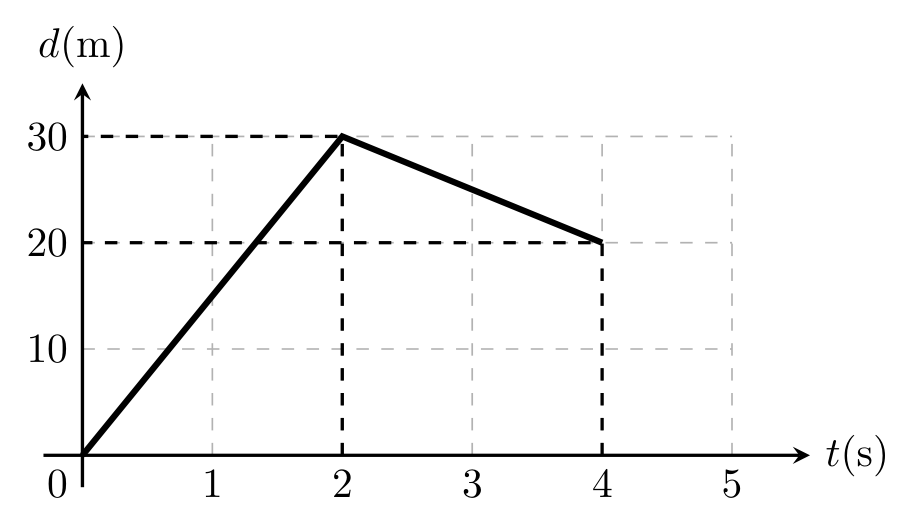
\includegraphics[width=6.2cm]{p3_c1_dothi.png}
		\vspace{-7pt}
	\end{center}

	\par\shortans[oly]{2}
	\loigiai{
		Từ đồ thị $d - t$ ta thấy:\\
		- Trong khoảng thời gian $t \in [0; 2\text{ s}]$: Độ dịch chuyển tăng từ $0$ đến $30\text{ m}$, vận tốc $v = \dfrac{30 - 0}{2 - 0} = 15\text{ m/s} > 0$, vật chuyển động theo chiều dương.\\
		- Trong khoảng thời gian $t \in [2\text{ s}; 4\text{ s}]$: Độ dịch chuyển giảm từ $30\text{ m}$ về $20\text{ m}$, vận tốc $v' = \dfrac{20 - 30}{4 - 2} = -5\text{ m/s} < 0$, vật chuyển động theo chiều âm.\\
		Như vậy, tại thời điểm $t = 2\text{ s}$, độ dịch chuyển đạt cực đại và vận tốc đổi dấu, tức là vật đổi chiều chuyển động.\\
		\textbf{Đáp số:} $2$.
	}
\end{ex}

% Phần III Câu 2
\begin{ex}
	\macau{ID: VL10-NH101-C24}Chạy marathon là một bộ môn thể thao dưới hình thức chạy bộ được ưa chuộng nhất trên thế giới, là một môn thể thao mang đến rất nhiều lợi ích cho sức khỏe. Người tham gia có thể chạy ở các cự ly $5\text{ km}$, $10\text{ km}$ hoặc $21\text{ km}$ rồi nâng lên đường chạy dài $42\text{ km}$ trong marathon. Tùy thuộc vào thể trạng mà chúng ta lựa chọn luyện tập ở cự ly phù hợp.
	
	Pace là một từ tiếng Anh được sử dụng để chỉ nhịp điệu trong chạy bộ. Pace là số phút để một người hoàn thành $1\text{ km}$ trong khi chạy. Bạn Hương mới tập luyện nên chọn cự ly $5\text{ km}$, trong một lần tập bạn đạt được thời gian hoàn thành cự ly $5\text{ km}$ là 42 phút. Pace trung bình trong bài luyện tập chạy bộ của bạn Hương là bao nhiêu phút/km?

	\par\shortans[oly]{8,4}
	\loigiai{
		Pace trung bình là số phút cần thiết để chạy được $1\text{ km}$:\\
		\[
		\text{Pace} = \frac{t}{s} = \frac{42\text{ phút}}{5\text{ km}} = 8{,}4\text{ phút/km}.
		\]
		\textbf{Đáp số:} $8{,}4$.
	}
\end{ex}

% Phần III Câu 3
\begin{ex}
	\macau{ID: VL10-NH101-C25}Đồ thị bên dưới mô tả sự thay đổi vận tốc theo thời gian trong chuyển động của một ô tô. Gia tốc của ô tô từ $t = 15\text{ s}$ đến $t = 30\text{ s}$ có giá trị bao nhiêu $\text{m/s}^2$?
	\begin{center}
		\vspace{-7pt}
		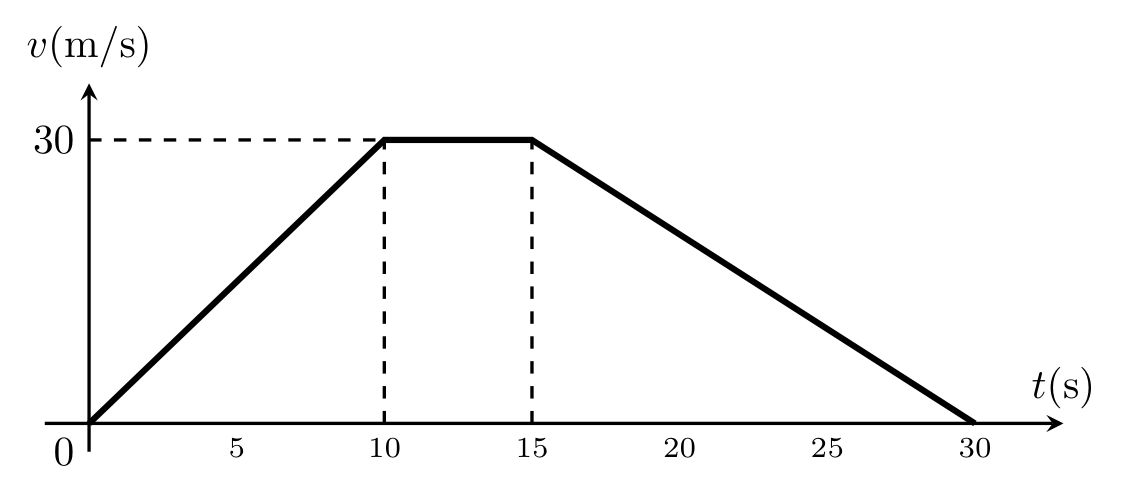
\includegraphics[width=6.6cm]{p3_c3_dothi.png}
		\vspace{-7pt}
	\end{center}

	\par\shortans[oly]{-2}
	\loigiai{
		Quan sát đồ thị $v - t$:\\
		- Tại thời điểm $t_1 = 15\text{ s}$, vận tốc của ô tô là $v_1 = 30\text{ m/s}$.\\
		- Tại thời điểm $t_2 = 30\text{ s}$, vận tốc của ô tô là $v_2 = 0\text{ m/s}$.\\
		Gia tốc của ô tô trong khoảng thời gian từ $t = 15\text{ s}$ đến $t = 30\text{ s}$ là:
		\[
		a = \frac{v_2 - v_1}{t_2 - t_1} = \frac{0 - 30}{30 - 15} = \frac{-30}{15} = -2\text{ m/s}^2.
		\]
		\textbf{Đáp số:} $-2$.
	}
\end{ex}

% Phần III Câu 4
\begin{ex}
	\macau{ID: VL10-NH101-C26}Một học sinh đo chiều dài của bàn học, kết quả thu được như sau $d = 120 \pm 1\text{ cm}$. Sai số tuyệt đối của phép đo trên là bao nhiêu cm?

	\par\shortans[oly]{1}
	\loigiai{
		Kết quả của phép đo được ghi dưới dạng chuẩn: $d = \overline{d} \pm \Delta d$.\\
		Trong đó $\overline{d} = 120\text{ cm}$ là giá trị trung bình, và $\Delta d = 1\text{ cm}$ là sai số tuyệt đối của phép đo.\\
		\textbf{Đáp số:} $1$.
	}
\end{ex}

% Phần III Câu 5
\begin{ex}
	\macau{ID: VL10-NH101-C27}Đồ thị bên dưới mô tả sự thay đổi vận tốc theo thời gian trong chuyển động của một vật. Vật thay đổi tính chất chuyển động từ chuyển động thẳng đều sang chuyển động thẳng biến đổi đều ở thời điểm nào (bao nhiêu giây)?
	\begin{center}
		\vspace{-7pt}
		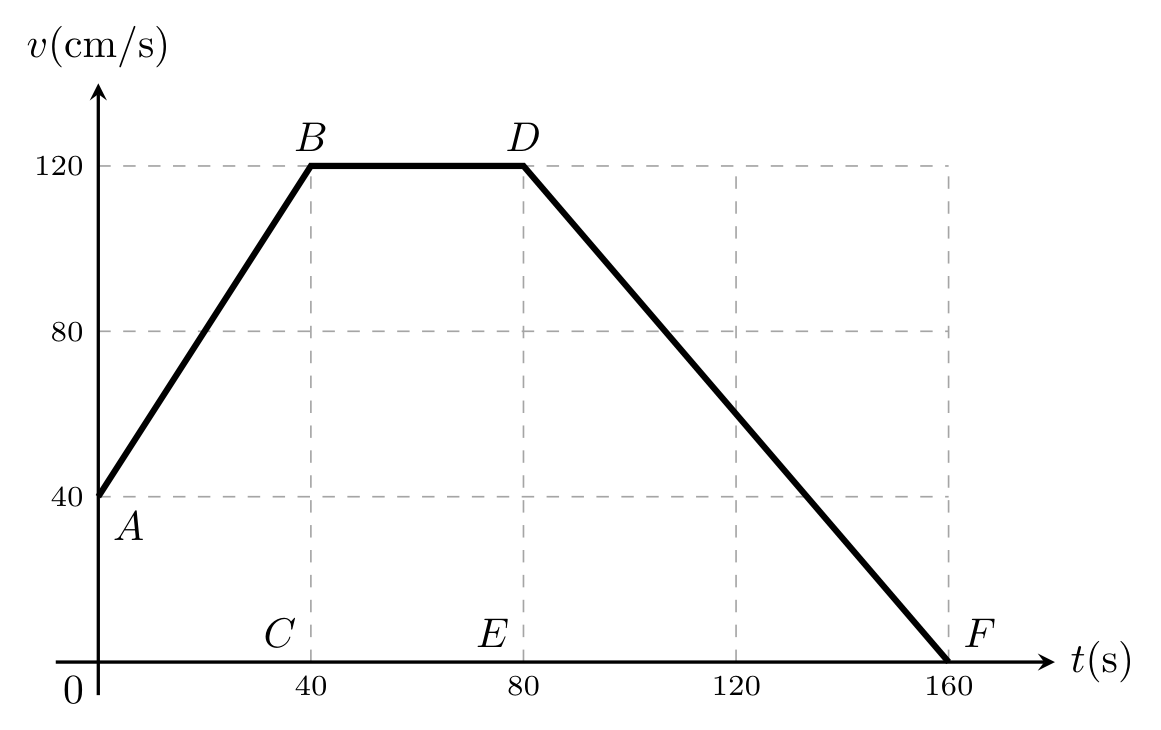
\includegraphics[width=7.2cm]{p3_c5_dothi.png}
		\vspace{-7pt}
	\end{center}

	\par\shortans[oly]{80}
	\loigiai{
		Phân tích đồ thị vận tốc -- thời gian:\\
		- Đoạn $AB$ ($0 \le t \le 40\text{ s}$): Đồ thị dốc lên, vận tốc tăng đều từ $40\text{ cm/s}$ đến $120\text{ cm/s}$ $\implies$ Chuyển động thẳng nhanh dần đều.\\
		- Đoạn $BD$ ($40\text{ s} \le t \le 80\text{ s}$): Đồ thị là đoạn nằm ngang, vận tốc không đổi $v = 120\text{ cm/s}$ $\implies$ Chuyển động thẳng đều.\\
		- Đoạn $DF$ ($80\text{ s} \le t \le 160\text{ s}$): Đồ thị dốc xuống, vận tốc giảm đều từ $120\text{ cm/s}$ về $0$ $\implies$ Chuyển động thẳng chậm dần đều (chuyển động thẳng biến đổi đều).\\
		Như vậy, tại điểm $D$ ứng với thời điểm $t = 80\text{ s}$, vật chuyển từ chuyển động thẳng đều sang chuyển động thẳng biến đổi đều.\\
		\textbf{Đáp số:} $80$.
	}
\end{ex}

% Phần III Câu 6
\begin{ex}
	\macau{ID: VL10-NH101-C28}Bạn Tuấn chạy bộ qua cầu đi thẳng $40\text{ m}$ theo hướng Đông, sau đó rẽ trái chạy thẳng theo hướng Bắc $100\text{ m}$ rồi quay ngược về hướng Nam $70\text{ m}$. Độ lớn độ dịch chuyển của Tuấn là bao nhiêu m?

	\par\shortans[oly]{50}
	\loigiai{
		Chọn hệ trục tọa độ $Oxy$ gắn với mặt phẳng ngang: gốc $O$ tại vị trí xuất phát, trục $Ox$ hướng về phía Đông, trục $Oy$ hướng về phía Bắc.\\
		- Lần 1: Đi thẳng $40\text{ m}$ hướng Đông: $\vec{d}_1 = (40; 0)\text{ m}$.\\
		- Lần 2: Rẽ trái đi $100\text{ m}$ hướng Bắc: $\vec{d}_2 = (0; 100)\text{ m}$.\\
		- Lần 3: Quay ngược về hướng Nam $70\text{ m}$: $\vec{d}_3 = (0; -70)\text{ m}$.\\
		Vectơ độ dịch chuyển tổng hợp của Tuấn là:
		\[
		\vec{d} = \vec{d}_1 + \vec{d}_2 + \vec{d}_3 = (40 + 0 + 0;\; 0 + 100 - 70) = (40; 30)\text{ m}.
		\]
		Độ lớn độ dịch chuyển tổng hợp là:
		\[
		d = |\vec{d}| = \sqrt{40^2 + 30^2} = \sqrt{1600 + 900} = \sqrt{2500} = 50\text{ m}.
		\]
		\textbf{Đáp số:} $50$.
	}
\end{ex}
